%\section{Grundlagen}
		\subsection{Trigonometrische Funktionen\color{red}S77-84 \color{black} Arcus\color{red}S86 \smallskip \color{black} Tabelle\color{red}S86}
			
%		\begin{multicols}{2}
%			\hspace{0pt}\scalebox{0.7}
%			{
%				$\begin{array}{c|c|c|c|c|c|c|c|c|c|c|c}
%				x & 0& 30 & 45& 60 & 90 & 120 & 135& 150& 180 & 270 & 360 \\ \hline
%				x & 0 & \pi / 6 & \pi / 4 & \pi / 3 & \pi / 2 & \frac{2}{3}\pi& \frac{3}{4}\pi& \frac{5}{6}\pi& \pi  & \frac{3}{2}\pi & 2 \pi \\ \hline
%				\sin & 0 & \frac{1}{2} & \frac{1}{\sqrt{2}} & \frac{\sqrt 3}{2} & 1 & \frac{\sqrt 3}{2} & \frac{1}{\sqrt{2}} & \frac{1}{2} & 0 & -1 & 0 \\
%				\cos & 1 & \frac{\sqrt 3}{2} & \frac{1}{\sqrt 2} & \frac{1}{2} & 0 & -\frac{1}{2} & -\frac{1}{\sqrt 2}  & -\frac{\sqrt 3}{2}   & -1 & 0 & 1 \\
%				\tan & 0 & \frac{\sqrt{3}}{3}&1 &\sqrt{3} & \pm \infty & -\sqrt{3}& -1& -\frac{1}{\sqrt{3}} & 0 & \pm \infty & 0\\
%				\cot & \pm \infty & \sqrt{3} & 1 & \frac{1}{\sqrt{3}} & 0 & -\frac{1}{\sqrt{3}} & -1 & -\sqrt{3} & \pm \infty & 0 & \pm \infty \\
%				\end{array}$
%			}
%		   
%			\paragraph{Trigometrische Wertebereiche}\
%			
%			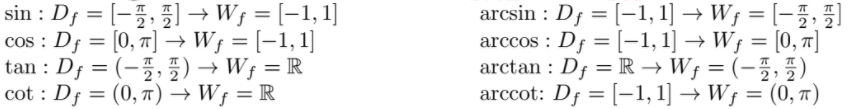
\includegraphics[width=7cm]{images/TrigFun.PNG}\\
%			
%		\end{multicols}
%
			\hspace{0pt}
			\begin{minipage}{0.55\columnwidth}
				\scalebox{0.7}{
				\begin{tabular}{c|c|c|c|c|c|c|c|c|c|c|c}
					x & 0& 30 & 45& 60 & 90 & 120 & 135& 150& 180 & 270 & 360 \\
					\hline
					x & 0 & $\frac{1}{6}\pi$ & $\frac{1}{4}\pi$ & $\frac{1}{3}\pi$ & $\frac{1}{2}\pi$ & $\frac{2}{3}\pi$& $\frac{3}{4}\pi$& $\frac{5}{6}\pi$& $\pi$  & $\frac{3}{2}\pi$ & $2 \pi $\\
					\hline
					$\sin$ & 0 & $\frac{1}{2}$ & $\frac{1}{\sqrt{2}}$ & $\frac{\sqrt 3}{2}$ & 1 & $\frac{\sqrt 3}{2}$ & $\frac{1}{\sqrt{2}}$ & $\frac{1}{2}$ & 0 & -1 & 0 \\
					$\cos$ & 1 & $\frac{\sqrt 3}{2}$ & $\frac{1}{\sqrt 2}$ & $\frac{1}{2}$ & 0 & $-\frac{1}{2}$ & $-\frac{1}{\sqrt 2}$  & $-\frac{\sqrt 3}{2}$   & -1 & 0 & 1 \\
					$\tan$ & 0 & $\frac{\sqrt{3}}{3}$&1 &$\sqrt{3}$ & $\pm \infty$ & $-\sqrt{3}$& -1& $-\frac{1}{\sqrt{3}}$ & 0 & $\pm \infty$ & 0\\
					$\cot$ & $\pm \infty$ & $\sqrt{3}$ & 1 & $\frac{1}{\sqrt{3}}$ & 0 & $-\frac{1}{\sqrt{3}}$ & -1 & $-\sqrt{3}$ & $\pm \infty$ & 0 & $\pm \infty$ \\
				\end{tabular}
				}
			\end{minipage}
			\hspace{3mm}
			\begin{minipage}{0.43\columnwidth}
				\textbf{Trigometrische Wertebereiche}\\[2pt]
				\scalebox{0.8}{
				\begin{tabular}{lcc|lcc}
					& $D_{f}$ & $W_{f}$ && $D_{f}$ & $W_{f}$\\
					\hline
					$\sin$ & $\left[\frac{-\pi}{2}, \frac{\pi}{2}\right]$ & $[-1,1]$ &
					$\arcsin$ & $[-1,1]$ & $\left[\frac{-\pi}{2}, \frac{\pi}{2}\right]$\\
					$\cos$ & $[0, \pi]$ & $[-1,1]$ & 
					$\arccos$ & $[-1,1]$ & $[0, \pi]$ \\
					$\tan$ & $\left(\frac{-\pi}{2}, \frac{\pi}{2}\right)$ & $\mathbb{R}$ &
					$\arctan$ & $\mathbb{R}$ & $\left(\frac{-\pi}{2}, \frac{\pi}{2}\right)$\\
					$\cot$ & $(0, \pi)$ & $\mathbb{R}$ &
					$\arccot$ & $[-1,1]$ & $(0, \pi)$
				\end{tabular}
				}
			\end{minipage}\\[5pt]
		
		
		\begin{tabulary}{14cm}{|L|L|L|L|}
			\hline
			$ \sin (-x) = -\sin (x) $ 							& $ \tan x = \frac{\sin x}{\cos x} $  &  $\sin \enbrace{x + \frac{\pi}{2}} = \cos x$ & $ \cos (x + y) = \cos x \cos y - \sin x \sin y $					\\ \hline
			
			$ \cos (-x) = \cos (x) $ 									& 	$\sin^2 x + \cos^2 x = 1$	 	& 	$\cos \enbrace{x - \frac{\pi}{2}} = \sin x$		&$\sin \enbrace{x + y} = \sin x \cos y + \cos x \sin y$	\\ \hline		
		\end{tabulary}\\

		$f(t)=A\cdot \cos(\omega t + \varphi_0)=A\cdot \sin(\omega t + \frac{\pi}{2}+ \varphi_0)$
		
	\vspace{1mm}
	\hrule
	\vspace{1mm}
		


		\begin{minipage}{0.37\textwidth}
			\subsection{Binomischer Satz \color{red} S12}%\  (fold)
			\label{par:fakultaeten}
			\begin{tabulary}{15cm}{Lccr}
				\fbox{$ (a+b)^{n}=\sum\limits_{i = 0}^{n}\binom{n}{i}a^{n-i}\cdot b^{i}  $} \qquad	&	
				\fbox{$ \binom{n}{i}= \frac{n!}{i!(n-i)!}  $}\qquad	& $\binom{n}{0} = \binom{n}{n} = 1$
				\qquad	& $ 2^{n}= \sum\limits_{i = 0}^{n}\binom{n}{i}  $\qquad\qquad 
				\\
			\end{tabulary}
		\end{minipage}%
		\vrule
		\hspace{2mm}
		\begin{minipage}{0.2\columnwidth}
				$ (a + b)^{2} = a^{2}+2ab+b^{2} $\\
				$ (a-b)^{2} = a^{2}-2ab+b^{2} $\\
				$ (a+b)(a-b) = a^{2}-b^{2} $\\
		\end{minipage}
		\\
		Bsp: $ (a+b)^{3}=\binom{3}{0}a^{3}\cdot b^{0} + \binom{3}{1}a^{2}\cdot b^{1}  +  \binom{3}{2}a^{1}\cdot b^{2}  +  \binom{3}{3}a^{1}\cdot b^{3}$  $ = 1a^{3}+3a^{2}\cdot b^{1}  +  3a^{1}\cdot b^{2}  +  1 b^{3}    $ 

	\vspace{1mm}	
	\hrule
	
	%----------------------------------------------------------------------------------------------------------------------------------------
		
%	\begin{multicols}{2}
%		\subsection{Logarithmus}
%			\begin{align*}
%				\ln(b)=x\Leftrightarrow e^{x}=b\Leftrightarrow e^{\ln(b)} &\qquad \log(b^{c})=c \cdot\log(b)\\
%				\log(b \cdot c)=\log(b)+\log(c) & \qquad \log(\dfrac{b}{c})=\log(b)-\log(c)\\
%				\dfrac{\lg(b)}{\lg(a)}=\dfrac{\ln(a)}{\ln(b)} & \lg(10)=1
%			\end{align*}
%		
%		\subsection{Potenzen}
%			\begin{align*}					%TODO_2: mit \begin{alignat*}{3} Tabelle zentrieren
%				a^{m} \cdot a^{n} = a^{m+n} & \qquad \dfrac{a^{m}}{a^{n}} = a^{m-n} & a^{0}=1
%				 \\
%				a^{n} \cdot b^{n} = \left(a \cdot b \right)^{n} & \qquad \dfrac{a^{n}}{b^{n}} = \left( \dfrac{a}{b} \right)^{n} & a^{-m} = \dfrac{1}{a^{m}}
%				\\
%				\left(a^{m}\right)^{n} = a^{m \cdot n}	& \qquad \left( \dfrac{a}{b} \right)^{-m} = \left( \dfrac{b}{a} \right)^{m}	& a^{1} = a
%				\\
%				1^{m} = 1 & \qquad 0^{m} = 0	&	
%			\end{align*}
%	\end{multicols}
%
%	\vspace{1mm}
\begin{minipage}[t]{0.49\columnwidth}
	\vspace{1mm}
	\subsection{Logarithmus {\color{red} S9}}
	\begin{tabular}{ll}
		$\ln(b)=x\Leftrightarrow e^{x}=b\Leftrightarrow e^{\ln(b)}$ & $\log(b^{c})=c \cdot\log(b)$\\[2mm]
		$\log(b \cdot c)=\log(b)+\log(c)$ & $\log\left(\dfrac{b}{c}\right)=\log(b)-\log(c)$\\[2mm]
		$\dfrac{\lg(b)}{\lg(a)}=\dfrac{\ln(a)}{\ln(b)}$ & $\ln(e)=1$ \\[4mm]
		$\lg(10)=1$ & $\ln(1)=0$\\
	\end{tabular}
	\vspace{1mm}
\end{minipage} \vline \hspace{0.02\columnwidth} 
\begin{minipage}[t]{0.49\columnwidth}
	\vspace{1mm}
	\subsection{Potenzen {\color{red} S9}}
	\begin{tabular}{lll}
		$a^{m} \cdot a^{n} = a^{m+n}$ & $\dfrac{a^{m}}{a^{n}} = a^{m-n}$ & $a^{0}=1$\\[2mm]
		$a^{n} \cdot b^{n} = \left(a \cdot b \right)^{n}$ & $\dfrac{a^{n}}{b^{n}} = \left( \dfrac{a}{b} \right)^{n}$ & $a^{-m} = \dfrac{1}{a^{m}}$\\[2mm]
		$\left(a^{m}\right)^{n} = a^{m \cdot n}$ & $\left( \dfrac{a}{b} \right)^{-m} = \left( \dfrac{b}{a} \right)^{m}$ & $a^{1} = a$\\[2mm]
		$1^m = 1$ & $0^m = 0$ & \\
	\end{tabular}
	\vspace{1mm}
\end{minipage}


	\hrule
	%----------------------------------------------------------------------------------------------------------------------------------------
	\vspace{1mm}
	
	\subsection{Ganzrationale Funktionen (Polynom $P(x)\in\mathbb R[x]_n$) \color{red}S63,65}
	\begin{tabular}{ll}
		$P(x)=\sum_{i=0}^n a_ix^i=a_n x^n+a_{n-1} x^{n-1}+\dotsc+a_1x+a_0$
		& $\bullet$ faktorisieren mit Hilfe von Binomen\\
		& $\bullet$ faktorisieren mit Hilfe des \textbf{Hornerschemas}{\color{red}S966}\\
	\end{tabular}
	\\
	\textbf{Wichtig:} eine ganzrationale Funktion $n$-ten Grades, hat höchstens $n$ verschiedene Nullstellen\\
	
	\begin{minipage}[b]{0.17\textwidth}
		\textbf{Polynomdivision {\color{red} S15}}\\
			Vorgehen:\quad Polynomdivision. $f$ der Asymptote kann aus dem Resultat gelesen werden.\\
			\\
			Beispiel:\qquad $f(x)=\dfrac{x^{3}+x+2}{3x}$ \\
			\\
			\\
			$\overset{Pol.Div.}{\Longrightarrow}$ \qquad 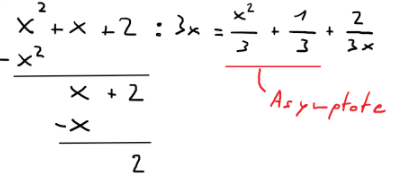
\includegraphics[width=3cm]{images/Skizze.png} \qquad\\
			%--------------------------------------------------------------------------------------------------------------------------------------------
			%		\hrule
			%		\subsubsection{Hornerschema \color{red}S966}
			%		\includegraphics[width=11cm]{images/Horner.PNG}\\
			%		%--------------------------------------------------------------------------------------------------------------------------------------------
			\textit{z.B.: Nulstelle: }\\
				 $ (-1) \Rightarrow :(x-(-1)) \iff \thickspace :(x+1) $\\
				 $ 3 \Rightarrow :(x-3)$\\[-6ex]
	\end{minipage}%
\hspace{1mm}
\vrule
\hspace{1mm}%
	\begin{minipage}[b]{0.33\textwidth}		
		\begin{minipage}[t]{0.3\textwidth}			
			\textbf{Mitternachtsformel \color{red} S41}\\[1ex]
				$ax^2+bx+c=0$ \\
				$x_{1,2}=\frac{-b\pm\sqrt{b^2-4ac}}{2a}$\\
	
			\textbf{pq-Formel}\\[1ex]
				$x^{2}+p x+q=0$\\			
				$x_{1,2}=-\frac{p}{2} \pm \sqrt{\left(\frac{p}{2}\right)^{2}-q}$\\
		\end{minipage}
		\hspace{1mm}
		\vrule
		\hspace{1mm}
		\begin{minipage}[t]{0.6 \textwidth}			
			\textbf{Satz von Vieta}\\[1ex]
				$ ax^2+bx+c=0 \quad \xLongrightarrow{:a} \quad x^{2}+p x+q=0 $ \\		
				   		
		   		Zusammenhänge: $ x_{1}+x_{2}=-p \qquad x_{1} \cdot x_{2}=q $	\\
		   		
		   %TODO_4: quadratische Ergänzung An für Dummies S.68
		   
		   \textbf{Gleichungen 3. und 4. Grades \color{red} S.42-43}\\[1ex]
		   \textit{siehe: Bronstein, S.42-43}
		\end{minipage}
	\\[1mm]
			\textbf{Diskriminante {\color{red} S41}} $\mathbb{L}\in \mathbb{R}$ \\
				\begin{equation*}
					D = b^{2}-4ac \quad \Rightarrow
					\begin{cases}
						 D > 0: & \text{2 Lösungen}\\
						 D = 0: & \text{1 Lösung}\\
						 D < 0: & \text{keine Lösung}\\
					\end{cases}
				\end{equation*}
		\end{minipage}


\vspace{1mm}
\hrule
%-----------------------------------------------------------------------------------------------------------------------------------------------------

	\subsection{Partialbruchzerlegung \color{red} S15}
\label{sub:allgemeines}



%Eine Funktion $f$ ist eine Abbildung, die jedem Element $x$ einer Definitionsmenge $D$ genau ein Element $y$ einer Wertemenge $W$ zuordnet.\\
$f(x)= \frac{-x^{2}+20x+149}{x^{3}+4x^{2}-11x-30} \Rightarrow$ Nenner Faktorisieren mit Hornerschema \color{red} S965 \color{black}, Binom\\ $x^{3}+4x^{2}-11x-30=(x+2)(x^{2}+2x-15)=(x+2)(x+5)(x-3)$ \\
Ansatz: $ f(x)= \frac{-x^{2}+20x+149}{x^{3}+4x^{2}-11x-30}=\frac{A}{x-3}+\frac{B}{x+2}+\frac{C}{x+5}=\frac{A(x+2)(x+5)+B(x-3)(x+5)+C(x+2)(x-3)}{(x-3)(x+2)(x+5)} $\\

Gleichungssystem (\textbf{Zähler gleichsetzten}) aufstellen mit beliebigen $x_{i}$-Werten (am Besten Polstellen oder 0, 1, -1 wählen):\\
\begin{tabulary}{12cm}{llll}
	
	$x_{1}=3$: 		& $-9+60+149=A\cdot 5\cdot 8$ 			& 	$\Rightarrow A=5$ 	&		\\
	$x_{2}=-2$:		&  $-4-40+149=B\cdot(-5)\cdot 3$ 		& 	$\Rightarrow B=-7$	&	$f(x)=\dfrac{5}{x-3}+\dfrac{-7}{x+2}+\dfrac{1}{x+5}$		\\ 
	$x_{3}=-5$: 	&  $-25-100+149=C\cdot (-8)\cdot (-3)$ 	& 	$\Rightarrow C=1$	&			\\
	
\end{tabulary}\\

weitere Ansätze für andere Typen von Termen:(Mehrere Werte für x verwenden, auch wenn kein Koeffizient 0 wird.)\\
\begin{tabulary}{1\textwidth}{ll}
Typ 1: $f(x)=\frac{5x^{2}-37x+54}{(x+1)(x-3)}=\frac{A}{x+1}+\frac{B}{x-3}$ 
& 
Typ 2: $f(x)=\frac{5x^{2}-37x+54}{(x+1)(x-3)^{2}}=\frac{A}{x+1}+\frac{B}{(x-3)^{1}}+\frac{C}{(x-3)^{2}}$\\ 
Typ 3: $f(x)=\frac{1}{x^{4}+x^{2}} = \frac{1}{x^{2}(x^{2}+1)}= \frac{A}{x^{1}}+\frac{B}{x^{2}}+ \frac{Cx+D}{x^{2}+1}$
\end{tabulary}

%-----------------------------------------------------------------------------------------------------------------------------------------------------
